\section{Conceptual Design}

The goal with this section is to describe the creative process
visually. First, I will describe the history behind the name, then
the icon, followed by the design choices made for the application itself.

\subsection{App Name}

The working name of the application has been GameList for years, even
before development began. It was simple and described what the
program did well enough.

The problem was that it lacked finesse, style, and a mascot. In order
to make your app good, it should have something simple, catchy, and
easy to say as its name. Google, Bing, Yahoo, or Wiki(pedia) are
great examples of a simple name that has style. GameList needed
to be changed into something better.

After consulting and thinking, I had nailed it down to what the name
should encompass:
\begin{itemize}
	\item A list or collection of things
	\item Related to gaming
	\item Involves time to complete
\end{itemize}

With that, me and M (anonymity protection) came together to make the name LoGL:

% TODO: Make it stand out on its own line
Library of Game Lengths.

There were a couple of other names that were possible as well to
achieve the same effect:
\begin{itemize}
	\item cataLog of Game Lengths
	\item List of Game Lengths
\end{itemize}

As an aside, I really liked this name because I created this program
to get rid of the gaming backlog. So LoGL can also be backLog of Game
Lengths. Once again, super fitting.

The program being called a LoGL and is easy, catchy, and fun to say.
Massive Win. With a new name obtained, it was now time to attach a
mascot for the app and icon.

\subsection{Icon}

With the name of the app being LoGL, it must relate to logs (wood
pieces) in some way.
Some animals to choose from were: squirrels, chipmunks, or beavers. I
opted for chipmunks because I think their cheeks filled with stuff is
cute. I also dislike squirrels. Beavers are brown and brown
isn't a fun app color. To choose a color for the chipmunk, M and I
looked asked a friend what they thought of when I said the new name,
and they said orange, which was exactly what M and I were thinking too.
As such, the mascot was an orange chipmunk.

The icon is a chipmunk with its cheeks filled with a game controller.
The goal was to make a cute icon which is indicative of what the
program is about. I think it works great!

\begin{figure}[htb]
	\centering
	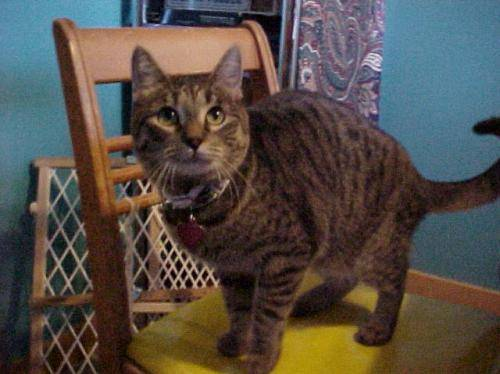
\includegraphics[width=10cm]{./Images/cats_00001.jpg}
	\caption{Photo of mascot}
	\label{fig:AppLD}
\end{figure}

% PERF: Give some backstory to the chipmunk like a name and stuff?

\subsection{Layout}

The goal of the layout was to make it simple, clean, and show the
user the top operations that would be used.
Labels were put next to icons that would be ambiguous for clarity.

For the rest of this section, I will assume that the user looks at
either the Light or Dark theme for reference.

\begin{figure}[htb]
	\centering
	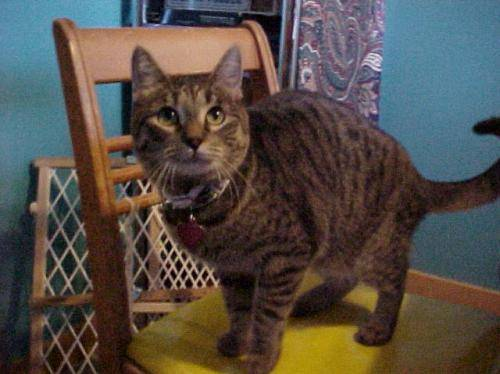
\includegraphics[width=10cm]{./Images/cats_00001.jpg}
	\caption{View of App in Light and Dark Mode}
	\label{fig:AppLD}
\end{figure}

\subsubsection{Main Window}

The main window has three elements in the layout:
\begin{enumerate}
	\item Toolbar
	\item Search bar
	\item Table (database)
\end{enumerate}

I will talk about them from top to bottom.
Before that however, it is important to talk about what happens when
the action causes an element to be created and be layered in front of
the contents of the current window, but still within it. An example is when
prompted with file selection. Instead of opening a new window, the
window gets a new layer on top with the new content, thus making the
contents of the lower layer unable to be interacted with. This is
different from when a new window is opened, which still allows the
user to interact with elements in the main window.

\begin{figure}[htb]
	\centering
	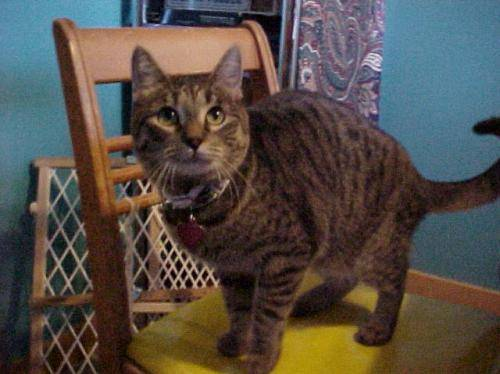
\includegraphics[width=10cm]{./Images/cats_00001.jpg}
	\caption{Comparison between popup vs new window}
	\label{fig:DBOperations}
\end{figure}

Referring back to the main app design in figure \ref{fig:AppLD}, I
will now describe it from the top down.

By making the colors of the buttons this color, the goal was to make
the highlight something that would stand out. By making it the
complement in the Light theme, this made it extremely apparent the
selection. In dark mode, I simply selected a light color that was
pretty to look at with high contrast.

When looking at the search bar, it was important to denote whether
the icon and text was a button or not. To show this, it lacks a
border like the buttons and instead is right next to the entry box
where the user can enter text to search for games. By being able to
differentiate the color of the search box and placeholder text, the
user can recognize easily that the search box is interactive, while
the label + icon is not.

The table has buttons as column headers which makes it easy to see that they
are interactive. The problem is that the table widget has an
unchangeable background color that persists in the top left corner,
and extends past the rows + columns if the window isn't large enough.
I can redefine the table widget, but I
actually think it helps separate the contents of the cells within the
table. If users don't like it, then of course it would be
possible to change it to match the background, or even make it
customizable, but for now it remains. In order to have more
clarity when looking at the table data, I wanted to make it alternate
between light and darker colors for each row. This would allow the
user to see different rows easily.

When the user clicks on a row, it has the same button hover
color which adds clarity and uniformity to the design.

\subsubsection{Settings Window}

The settings window lists each option separated by a black line. The
goal was to show the user that each option is clearly different from
the next. I opted to leave the settings in the order they would
probably be most used in, top to bottom.

\begin{figure}[htb]
	\centering
	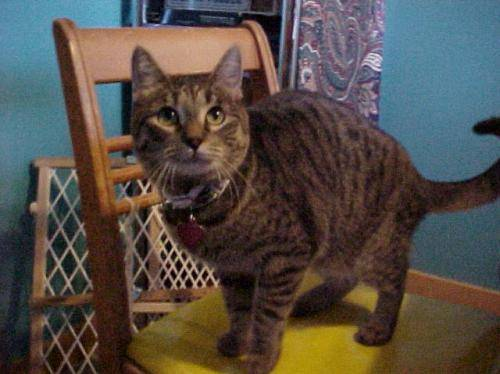
\includegraphics[width=10cm]{./Images/cats_00001.jpg}
	\caption{Settings Menu Light/Dark}
	\label{fig:DBOperations}
\end{figure}

The selector radio highlights where the user hovers their cursor over
the option. This shows the app is responsive which is always a plus.
This is also visible on the slider for the Text and Icon size.

\subsection{Icons}

By using icons that were built into the fyne and developing only one
icon myself (the heart SVG seen in section \ref{subsubsec:Assets}), I
was able to implement icons that are familiar to the user, and only
add text to those that were unclear as to what they meant.

The list of icon shapes and their uses are listed below:
\begin{itemize}
	\item Triangle (ASC sort order)
	\item Inverted Triangle (DESC sort order)
	\item Plus Sign (Add)
	\item Circular Arrow (Update)
	\item Minus Sign (Remove)
	\item Magnifying Glass with Arrows (Random Row)
	\item Heart (Un/Favorite)
	\item Paper Airplane (Export)
	\item Question Mark (Help)
	\item Gear (Settings)
\end{itemize}

The icons can be viewed in this graphic below without modification:

\begin{figure}[htb]
	\centering
	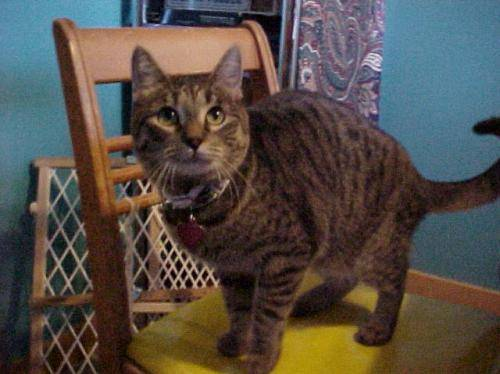
\includegraphics[width=10cm]{./Images/cats_00001.jpg}
	\caption{Show all icons together}
	\label{fig:DBOperations}
\end{figure}
